\chapter*{APPENDIX}
\phantomsection
\addcontentsline{toc}{chapter}{APPENDIX}
\setcounter{secnumdepth}{0}

This appendix documents the synthetic control construction methodology considered during the thesis design. It summarizes the control basket, weight construction, hold-out validation, and the reason Cumulative Abnormal Returns (CAR) was not retained as the main outcome.

\section{Control Basket Composition}
\label{sec:app-control-basket}

The default macro-market control basket consisted of eight major cryptocurrency assets selected to represent broad market movements natively decoupled from specific micro-cap pump manipulation influences.

\begin{table}[htbp]
\centering
\caption{Synthetic Control Macro-Market Basket Composition}
\label{tab:app-control-basket}
\begin{tabular}{|l|l|p{6.5cm}|}
\toprule
\multicolumn{1}{|c|}{\textbf{Asset}} & \multicolumn{1}{c|}{\textbf{Ticker}} & \multicolumn{1}{c|}{\textbf{Selection Rationale}} \\
\midrule
Bitcoin & BTC & Market benchmark, high liquidity \\
Ethereum & ETH & Smart contract platform leader \\
Binance Coin & BNB & Exchange token, Binance ecosystem \\
Ripple & XRP & Cross-border payments focus \\
Cardano & ADA & Proof-of-stake platform \\
Solana & SOL & High-throughput blockchain \\
Litecoin & LTC & Legacy altcoin, long history \\
Chainlink & LINK & Oracle network, DeFi infrastructure \\
\bottomrule
\end{tabular}
\datasetsource
\end{table}

\section{Weight Optimization via Constrained Least Squares}

The methodology theoretically constructed the counterfactual as a weighted average of control unit returns implementing a Constrained Least Squares (CLS) logic that optimized direct return-matching across defined prior validation windows.

To systematically prevent data contamination and arbitrary overfitting, testing utilized discrete trailing periods anchored prior to the $T_0$ signal event.
\begin{itemize}
    \item \textbf{Training Window}. $[min(T_0 - 84\text{h}), T_0 - 36\text{h}]$ (optimized CLS control array alignments)
    \item \textbf{Hold-Out Window}. $[T_0 - 36\text{h}, T_0 - 12\text{h}]$ (out-of-sample parametric $R^2$ validation tracking evaluation)
\end{itemize}

A formal 12-hour gap directly preceding explicit manifestation at $T_0$ prevented potential preliminary internal coordination leaks from corrupting empirical baseline assessments.

The weight vector $\boldsymbol{\omega}$ ensured that synthesized baseline evaluations hypothetically represented a realistic portfolio through standard weight constraints.

\begin{equation}
    \min_{\boldsymbol{\omega}} \| \mathbf{y} - \mathbf{X}\boldsymbol{\omega} \|_2^2
    \quad \text{subject to} \quad
    \sum_{k} \omega_k = 1, \quad \boldsymbol{\omega} \geq 0
\end{equation}

where $\mathbf{y}$ is the vector of returns for the target coin during the training window, $\mathbf{X}$ is the matrix of returns for the macro-market control basket, and $\boldsymbol{\omega}$ is the vector of weights assigned to each control asset. The constraints ensure the synthetic control is a fully invested ($\sum \omega_k = 1$) and long-only ($\boldsymbol{\omega} \geq 0$) portfolio.

The optimization used logarithmic returns because absolute prices are not stationary over time. This approach prevented small discrepancies in price trends from causing the synthetic control and target coin paths to drift apart during multi-day evaluations.

\section{Hold-Out Tracking Validation Results}
\label{sec:app-hold-out-validation}

Out-of-sample validation tests showed that micro-cap markets often move independently from the broader economy.

\begin{table}[htbp]
\centering
\caption{Distribution of \textit{Hold-Out $R^2$} Tracking Validation Metrics (N=3,320 Events)}
\begin{tabular}{|l|r|r|r|r|r|}
\toprule
\multicolumn{1}{|c|}{\textbf{Metric}} & \multicolumn{1}{c|}{\textbf{Mean}} & \multicolumn{1}{c|}{\textbf{Median}} & \multicolumn{1}{c|}{\textbf{P25}} & \multicolumn{1}{c|}{\textbf{P75}} & \multicolumn{1}{c|}{\textbf{Std Dev}} \\
\midrule
\textit{Hold-Out $R^2$} & 0.092 & $-$0.003 & $-$0.031 & 0.200 & 0.227 \\
\bottomrule
\end{tabular}
\datasetsource
\end{table}

The near-zero median correlation indicates that coins targeted by pump-and-dump groups are generally not driven by typical market-wide trends.
\section{Limitations of Cumulative Abnormal Returns (CAR)}
\label{sec:app-car-limitations}

Initially, this study used Cumulative Abnormal Returns (CAR) to try and isolate the coin's performance from broader market movements.
\begin{equation}
CAR_{i,\Delta} = r_{target,i}^{[0,\Delta]} - r_{control,i}^{[0,\Delta]}
\label{eq:car-original}
\end{equation}
where $r_{target}^{[0,\Delta]}$ is the actual log-return and $r_{control}^{[0,\Delta]}$ is the synthetic estimate of what the price would have been without the pump.

However, this method did not work well for our sample. As shown in Figure~\ref{fig:app-r2-distribution}, the average $R^2$ between synthetic controls and actual prices was close to zero. The model failed to predict prices accurately for the micro-cap and small-cap coins that pump-and-dump groups typically target.

\begin{figure}[htbp]
\centering
\caption{Distribution of $R^2$ scores across \textit{Market Capitalization} strata. The scores are consistently near zero, showing that synthetic controls cannot accurately track micro-cap assets.}
\label{fig:app-r2-distribution}
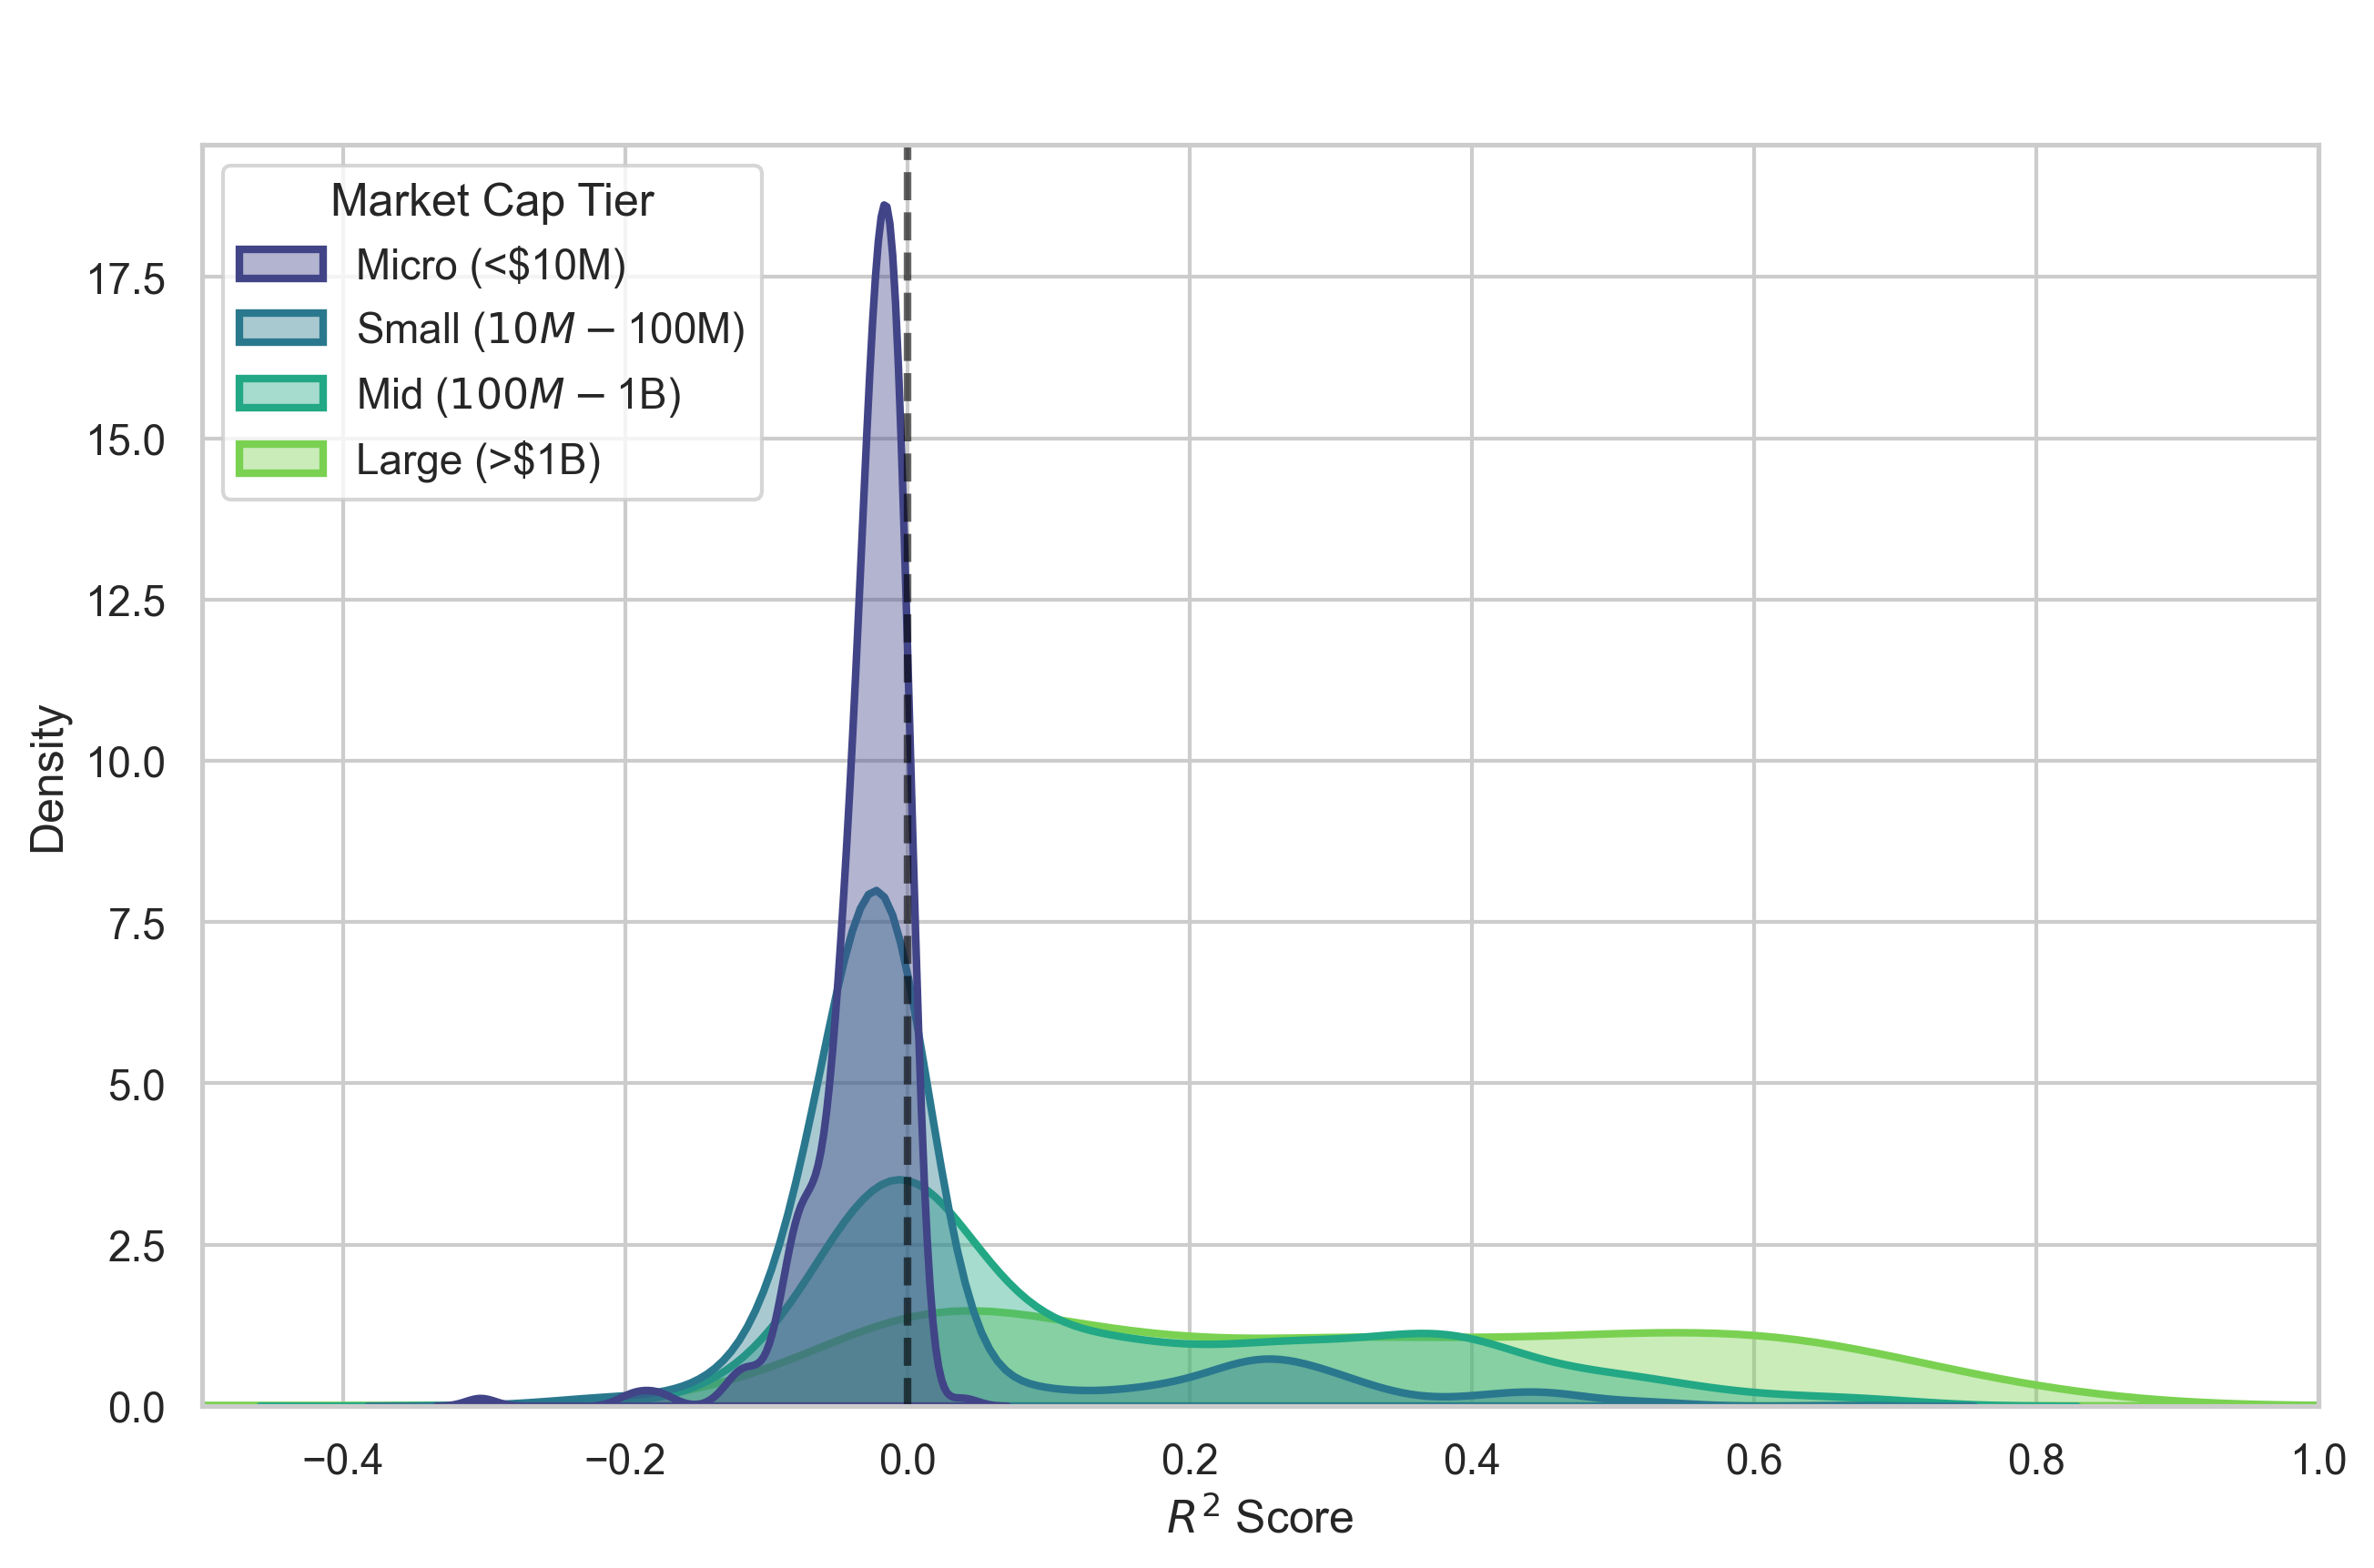
\includegraphics[width=0.8\textwidth]{figures/ch4/r2_distribution_by_mcap.png}
\source{Own elaboration based on the thesis dataset. Note: \textdollar{} denotes USD; M denotes million; B denotes billion.}
\end{figure}

Because the synthetic controls failed to track the target coins, using CAR actually made the results less reliable. Instead of removing market noise, subtracting an unrelated control variable just added more variance to the data.
\begin{equation}
\text{Var}(CAR) = \text{Var}(r_{target}) + \text{Var}(r_{control}) - 2\text{Cov}(r_{target}, r_{control})
\end{equation}
When the two variables are completely unrelated (zero covariance), CAR results in higher variance than the original returns. This extra noise can hide the true statistical effects of the pump.

If we had filtered the sample to only include cases where the synthetic control worked (e.g., $R^2 > 0.25$), we would have lost over 75\% of our data. More importantly, this would have removed almost all low-liquidity and micro-cap coins. This would have shifted our focus entirely to large-cap assets that are rarely affected by these groups. For these reasons, it was decided not to use CAR. Instead, the standard logarithmic returns were used and market conditions were handled directly within the Double Machine Learning models.
